\section{Theoretical Background \& Related Work}
\label{sec:background}

\paragraph{Notation.} We denote \(T_p\) and \(T_f\) as the numbers of observed and predicted timesteps, respectively. Following UniTraj conventions~\cite{unitrajFeng2024}, agent trajectories are represented as \(\boldsymbol{X}_d \in \mathbb{R}^{N_{\max} \times T_p \times F_{ap}}\) and map polylines as \(\boldsymbol{X}_s \in \mathbb{R}^{K_{\max} \times L \times F_{map}}\), where \(N_{\max}\) is the maximum number of agents, \(K_{\max}\) is the maximum number of map polylines, \(L\) is the points per polyline, and \(F_{ap}, F_{map}\) are the respective feature dimensions. Ground truth trajectories for the center agent are denoted \(\boldsymbol{y}_c \in \mathbb{R}^{T_f \times 4}\). For rasterized approaches, BEV representations use \(H \times W\) spatial resolution with \(F_d, F_s\) channel dimensions for dynamic and static inputs, respectively. Transformer models employ \(M\) output modes, \(K\) sampling points per deformable attention query, and \(N\) attention heads. Feature pyramid networks utilize \(L\) levels indexed by \(\ell \in \{0,\dots,L-1\}\), with feature maps \(C_\ell \times H_\ell \times W_\ell\) at each level. A comprehensive symbol table is provided in Appendix~\ref{app:notation}.

\subsection{Rasterized BEV and CASPNet}
Rasterized models convert trajectories and HD maps into BEV image stacks:
\[
I_d\in\mathbb{R}^{T_p\times H\times W\times F_d},\quad
I_s\in\mathbb{R}^{H\times W\times F_s}.
\]
These are encoded with parallel FPN backbones and fused temporally via ConvLSTM~\cite{caspnetSchäfer2022,arXiv:2201.06933v1}.

\begin{figure}[ht]
  \centering
  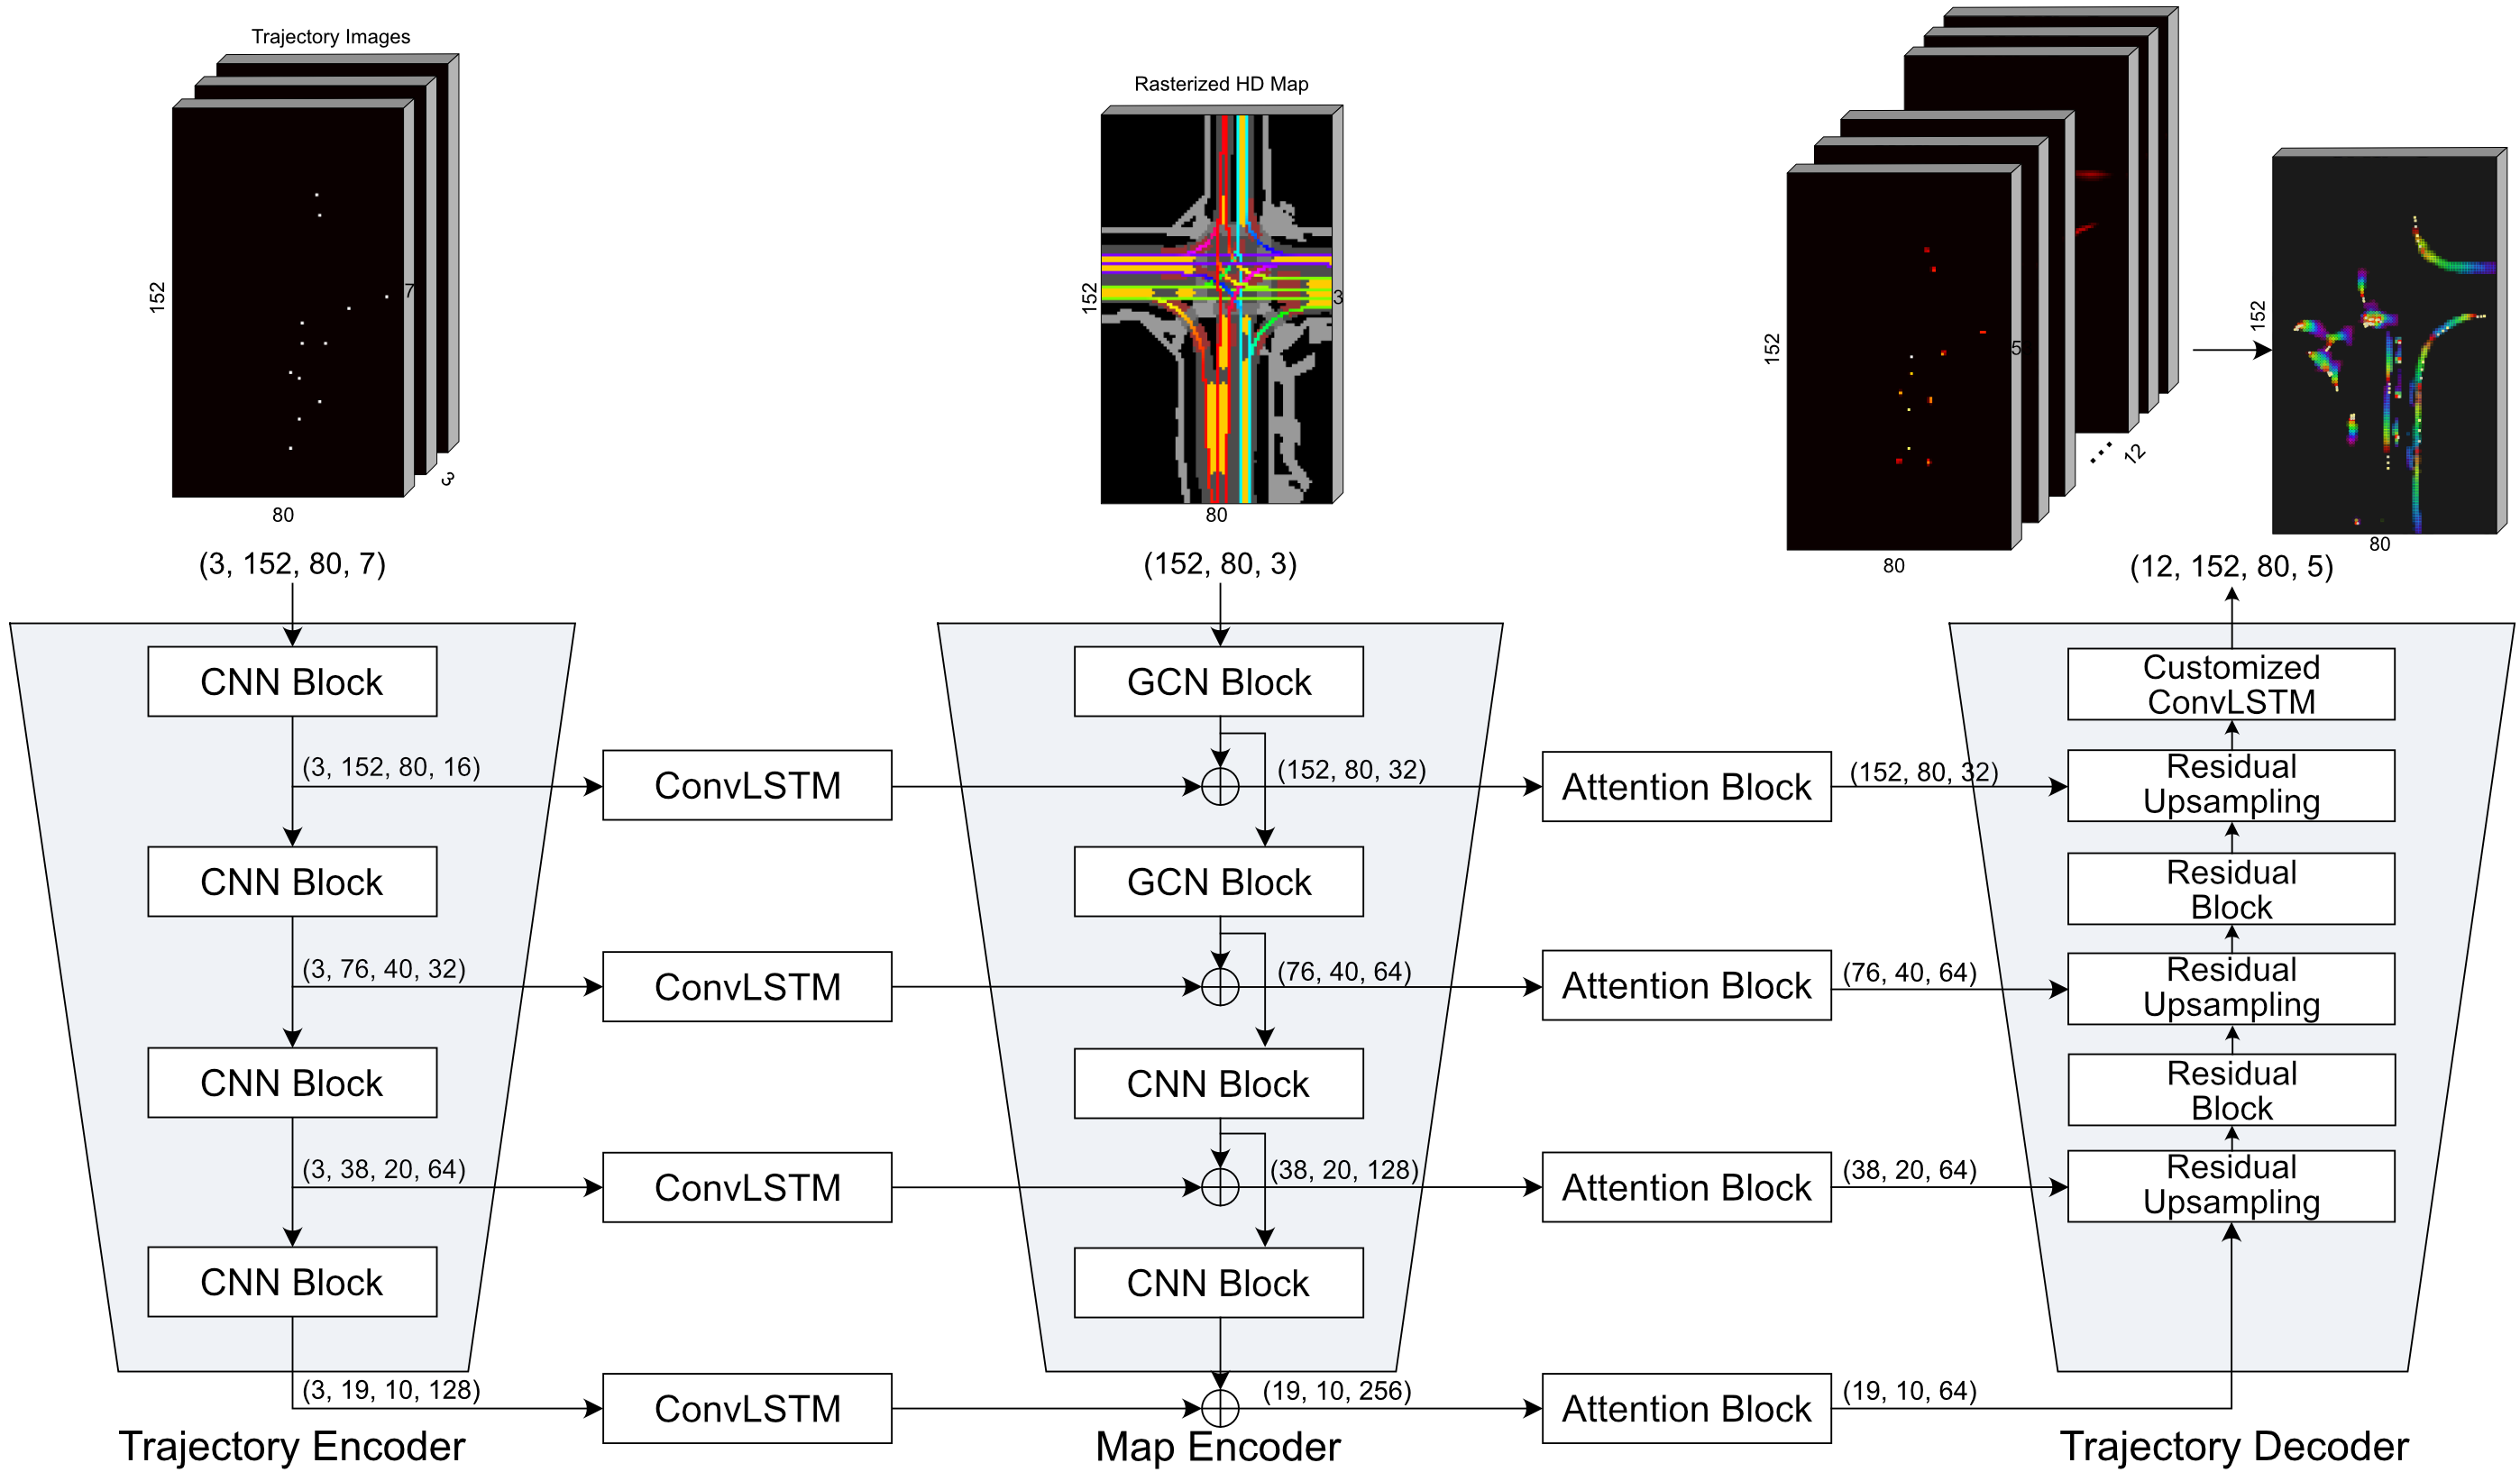
\includegraphics[width=\linewidth]{figures/caspnet_arch.png}
  \caption{CASPNet architecture: dual FPN encoders, pixel-adaptive attention, residual upsampling, and ConvLSTM decoder.}
  \label{fig:caspnet_overview}
\end{figure}

\paragraph{FPN Encoding.} At each level $\ell$, the trajectory branch produces
\[
F_{\ell}^{\mathrm{traj}}
= \mathrm{ConvLSTM}_\ell\Bigl\{\mathrm{CNN}_\ell\bigl(I_d(t)\bigr)\Bigr\}_{t=1}^{T_p},
\]
and the map branch
\[
F_{\ell}^{\mathrm{map}}
= \mathrm{CNN}_\ell^{\mathrm{Gabor}}(I_s).
\]
These form $\mathcal F=\{F_\ell^{\mathrm{traj}}\oplus F_\ell^{\mathrm{map}}\}_{\ell=0}^{L-1}$.

\paragraph{Pixel-Adaptive Attention.} To flexibly capture interactions at varying ranges, each fused feature map $X\in\mathbb R^{g\times h\times k_{\mathrm{in}}}$ is processed via dilated convolutions and learned attention weights:
\[
W(X)=\mathrm{softmax}\bigl(\mathrm{Conv}_{\mathrm{att}}(X)\bigr)\in\mathbb R^{g\times h\times n},
\]
\[
X_{\mathrm{out}}(x,y) = \sum_{i=1}^n W_i(x,y)\,\bigl[\mathrm{Conv}_{d_i}(X)\bigr](x,y),
\]
where $d_1<\dots<d_n$ are dilation rates.
\begin{figure}[ht]
  \centering
  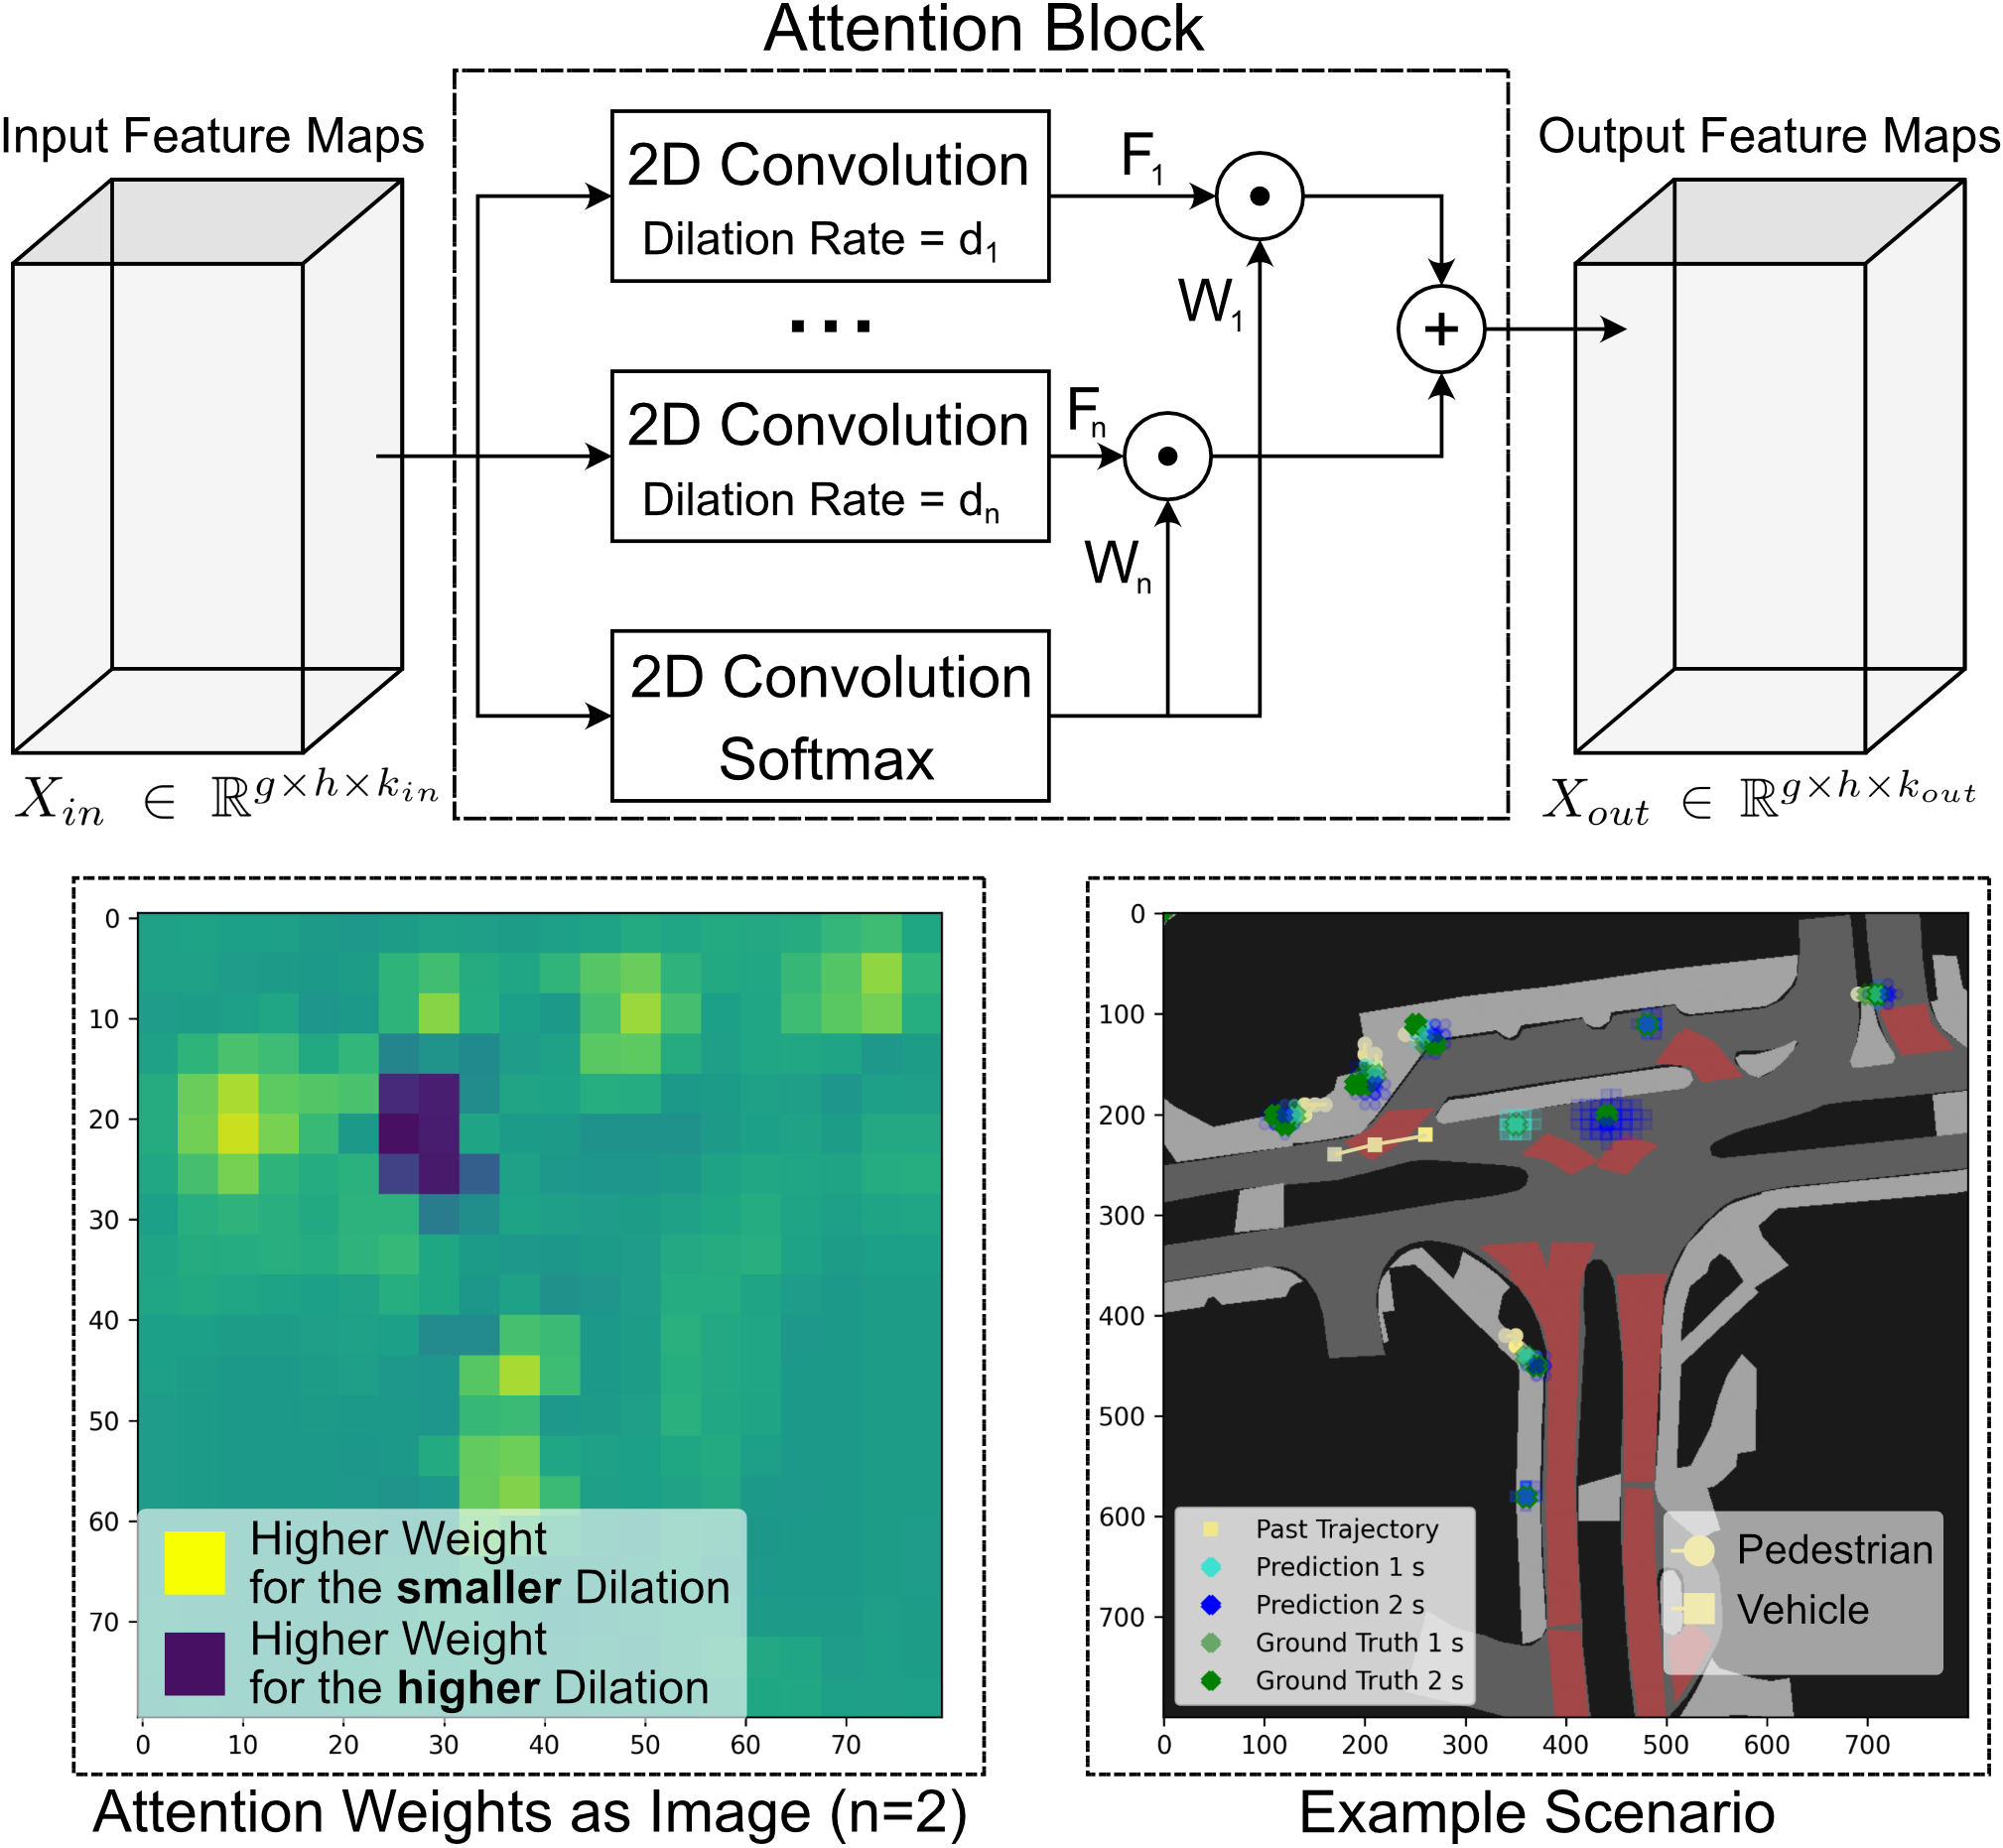
\includegraphics[width=\linewidth]{figures/caspnet_attn_block.png}
  \caption{Pixel-adaptive attention: learned per-pixel weights on multi-dilated convolutions.}
  \label{fig:attention_block}
\end{figure}

\paragraph{Residual Upsampling \& ConvLSTM Decoder.} Features are upsampled via
parallel bilinear and transposed-conv branches plus a residual Inception block, then concatenated across levels. A ConvLSTM then {\it unfolds} along $t=1,\dots,T_f$:
\[
H_t = \mathrm{ConvLSTM}\bigl(U(H_{t-1}),H_{t-1}\bigr),\quad
O_t = \mathrm{softmax}\bigl(W_o H_t + b_o\bigr),
\]
yielding per-pixel occupancy and in-pixel offsets for all $t$ in one forward pass.

\paragraph{Gaussian-Kernel Supervision.} Ground truth at pixel $(u,v)$ for class $c$ at time $t$ is smoothed via a 2D Gaussian:
\[
Y_{tuvc} = \exp\!\Bigl[-\tfrac12(\mathbf{p}_{uv}-\mathbf{p}^*_t)^\top\Sigma_t^{-1}(\mathbf{p}_{uv}-\mathbf{p}^*_t)\Bigr],
\]
where $\mathbf{p}^*_t$ is the true position, and $\Sigma_t$ grows with $t$ and speed $v_t$.

\paragraph{Training Losses \& Limitations.} Training combines:
- A distance-aware focal loss~\cite{Law_2018_ECCV} on $O_{tuvc}$ to address class imbalance;
- A masked $\ell_2$ regression loss on in-pixel offsets at positive locations.
While CASPNet excels in scalable joint prediction, it suffers from BEV quantization and lacks explicit vectorized outputs for downstream modules.

% --- Gabor Filter Steerability and Isomorphisms paragraph inserted here ---

\paragraph{Gabor Filter Steerability and Isomorphisms.}
Gabor filters are defined by a sinusoidal plane wave modulated by a Gaussian envelope:
\[
G_{\lambda,\theta,\psi,\sigma,\gamma}(x,y)
= \exp\!\Bigl(-\tfrac{x'^{2} + \gamma^{2}y'^{2}}{2\sigma^{2}}\Bigr)
  \cos\!\Bigl(2\pi \tfrac{x'}{\lambda} + \psi\Bigr),
\]
where
\(
x' = x\cos\theta + y\sin\theta,\;
y' = -x\sin\theta + y\cos\theta,
\)
and $\lambda$ (wavelength), $\theta$ (orientation), $\psi$ (phase), $\sigma$ (scale), and $\gamma$ (aspect ratio) control the filter's frequency and spatial extent~\cite{gabor}.
Crucially, Gabor filters are \emph{steerable}: any rotated version can be expressed as a linear combination of a finite set of basis filters:
\[
G_{\lambda,\theta}(x,y)
= \sum_{n=1}^N k_n(\theta)\,G_{\lambda,\theta_n}(x,y),
\]
with fixed prototype orientations~$\{\theta_n\}$ and interpolation coefficients~$\{k_n(\theta)\}$.
This steerability property induces an isomorphism between the continuous rotation group $\mathrm{SO}(2)$ and the subspace spanned by the basis filters: the group operation of rotation corresponds exactly to matrix multiplication of the basis coefficients $\mathbf{k}(\theta)$, yielding an equivalent representation in filter space.
Similarly, sampling $\sigma$ at multiple scales yields an isomorphism to the positive real scaling group $\mathbb{R}^+$.
Together, steerable Gabor filters implement an approximation of a group convolution over the Euclidean similarity group $\mathrm{SIM}(2)\!=\!\mathbb{R}^2\rtimes(\mathrm{SO}(2)\times\mathbb{R}^+)$, endowing the resulting feature maps with equivariance to translations, rotations, and dilations.

\subsection{Transformer-Based Vectorized Forecasting and CASPFormer}
Vectorized models predict explicit $(x,y)$ trajectories via transformer decoders, leveraging deformable attention to maintain efficiency~\cite{zhu2021deformabledetr,arXiv:2409.17790v1}.

\paragraph{Deformable MSDA.} Each query $q$ attends to $K$ sampling points across multiple feature levels:
\[
p_{q\ell k}=p_q + \Delta p_{q\ell k},\quad
\mathrm{MSDA}(Q,K,V)
= \sum_{\ell=0}^{L-1}\sum_{k=1}^K A_{q\ell k}\,W_\ell\,V_\ell(p_{q\ell k}),
\]
where $\Delta p$ are learned sampling offsets and $A_{q\ell k}$ are attention weights. This mechanism enables efficient multi-scale feature fusion at linear complexity while maintaining the ability to capture both local and global context from BEV representations.

\paragraph{Reference Point Mechanism.} A crucial aspect of CASPFormer's deformable cross-attention is the reference point initialization and updating strategy. The ego vehicle position serves as the initial reference anchor, providing spatial grounding for the attention mechanism. Although ablation studies show that ego-vehicle positioning does not significantly improve single-agent prediction performance, this mechanism is designed to facilitate future extensions to multi-agent joint prediction scenarios where agent-specific reference points become critical for modeling interactions.

\subsubsection{CASPFormer Architecture}
\begin{figure}[ht]
  \centering
  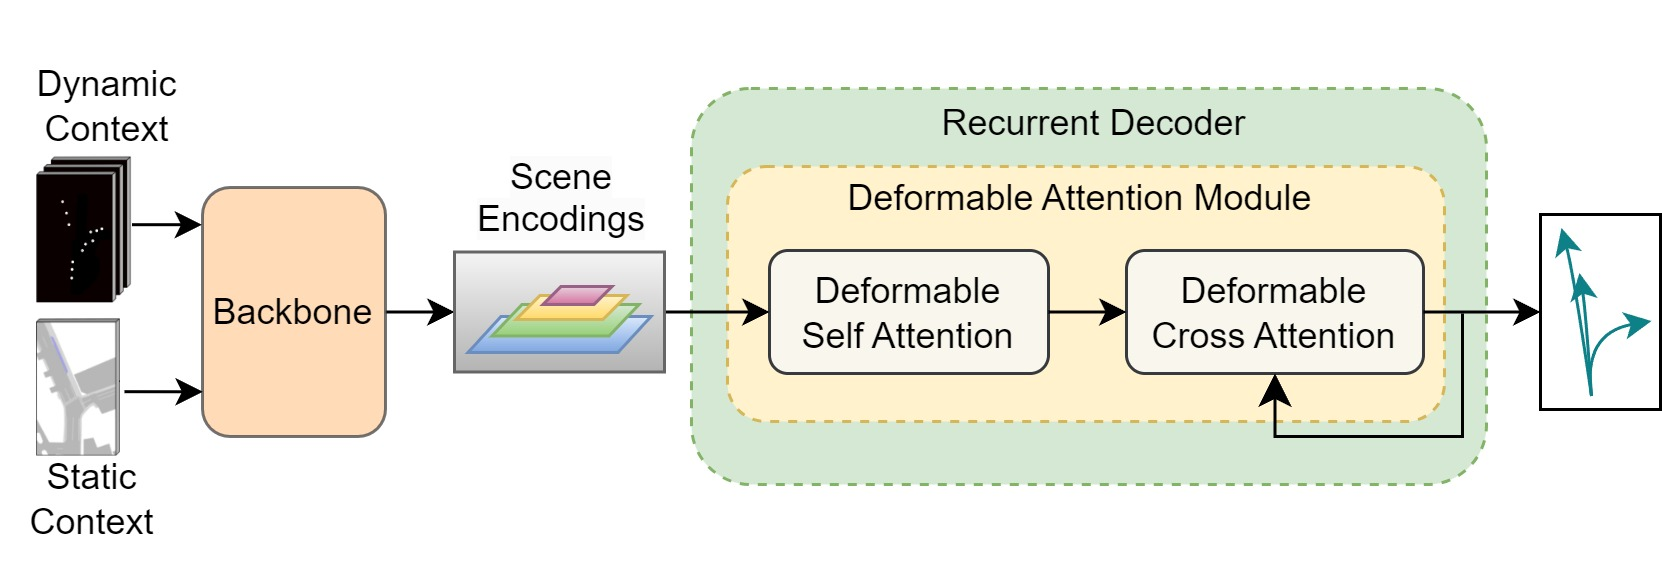
\includegraphics[width=\linewidth]{figures/caspformer-overall-arch.jpg}
  \caption{CASPFormer: BEV-CNN backbone, MSDA fusion, and recurrent CrossDA decoder with dual queries.}
  \label{fig:caspformer_overall}
\end{figure}

CASPFormer retains CASPNet's proven CNN backbone but replaces the grid-based decoder with a sophisticated transformer architecture that directly outputs vectorized trajectories. The CNN backbone + FPN yields multi-scale tokens $\{F_\ell\}$, which are spatially flattened and enriched with 2D sinusoidal position embeddings before being fused by MSDA into $Z\in\mathbb R^{N\times d}$.

\paragraph{Dual-Query Architecture.} A key innovation of CASPFormer is its dual-query system that addresses fundamental challenges in multimodal trajectory prediction. Contrary to previous studies~\cite{girgis2021latent,varadarajan2022multipath++,zhou2023query} which use a single set of learnable embeddings, CASPFormer employs two complementary query mechanisms:
\begin{itemize}
\item \emph{Temporal queries} $T_t$ capture sequential dependencies across time steps through recurrent feedback loops, enabling temporal coherence in predicted trajectories
\item \emph{Mode queries} $M$ are fixed learnable embeddings that explicitly combat mode collapse by representing distinct behavioral patterns and encouraging trajectory diversity
\end{itemize}
The final decoder query is formed by element-wise summation: $Q_t = T_{t-1} + M$.

\paragraph{Mode Collapse Mitigation.} Initial experiments using only temporal queries resulted in mode collapse, where different modes corresponded primarily to different speeds while missing other scene-consistent trajectories (e.g., different lane choices or turning behaviors). The introduction of dedicated mode queries significantly improves trajectory diversity and ensures that each mode learns to represent distinct behavioral patterns, as demonstrated in the original paper's qualitative results.

The recurrent decoder maintains:
\[
Q_t = T_{t-1} + M,\quad
Y_t = \mathrm{CrossDA}(Q_t,Z,r_{t-1}),
\]
with
\[
\mathrm{CrossDA}(Q,Z,r)
=\sum_{\ell,k}A^{\mathit{x}}_{\ell k}\,W_\ell\,Z_\ell(r+\Delta p_{\ell k}).
\]
Outputs $Y_t$ update both the reference point and temporal queries:
\[
r_t = r_{t-1} + \delta_r(Y_t),\quad
T_t = \phi(Y_t),
\]
ensuring spatial anchoring around the ego vehicle position and temporal coherence across prediction steps.
\begin{figure}[ht]
  \centering
  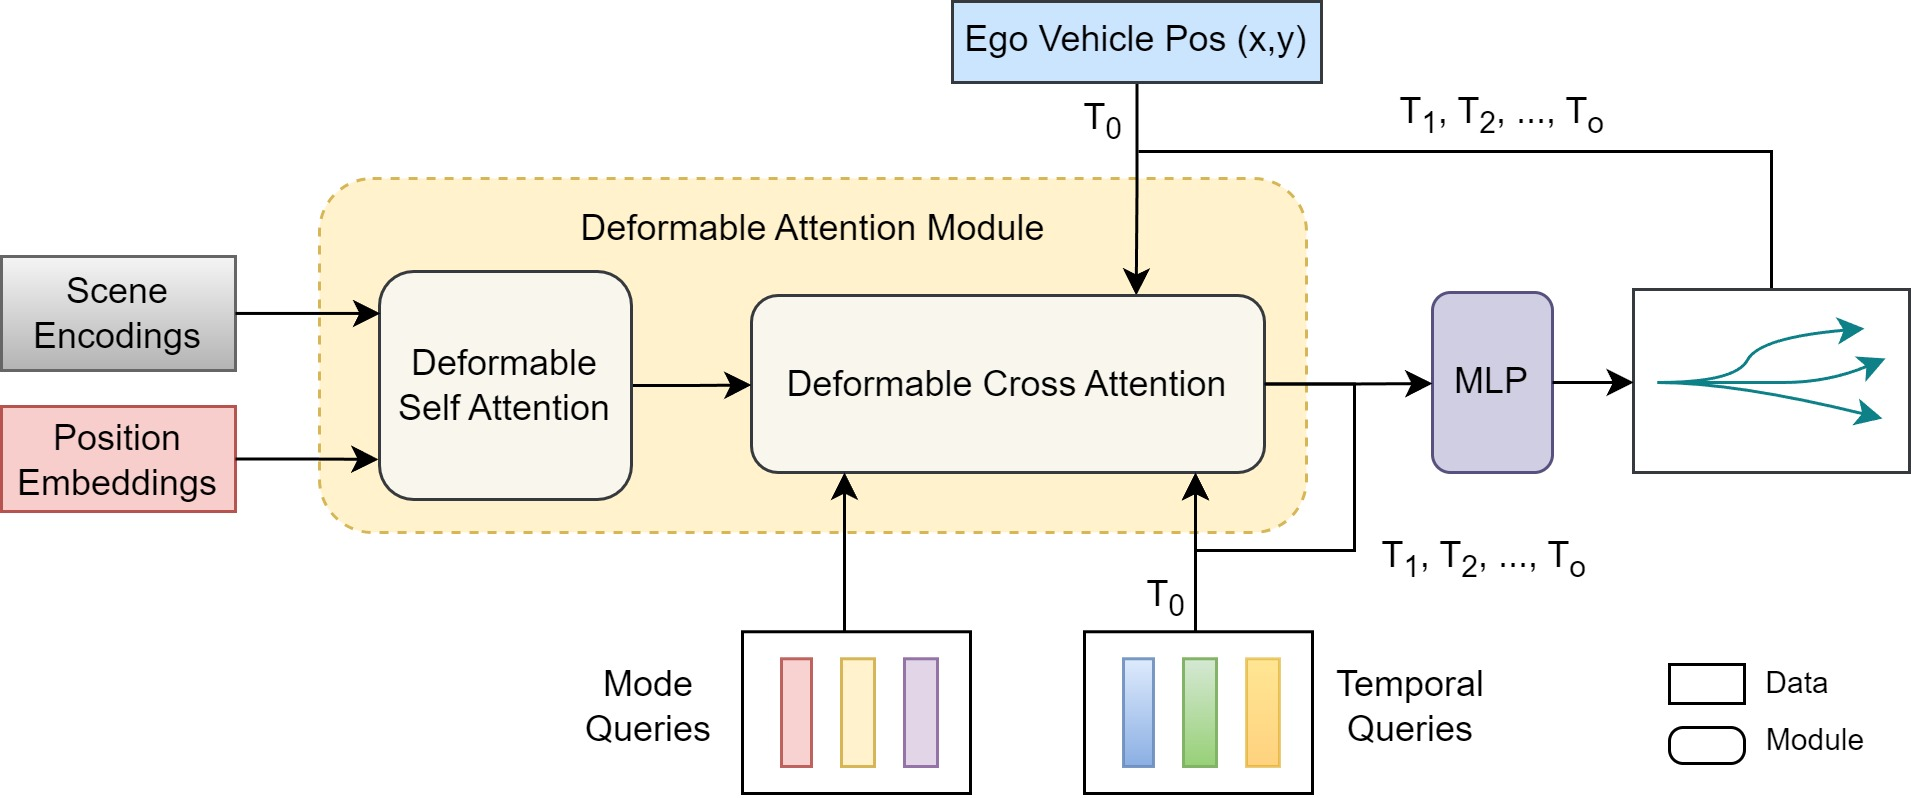
\includegraphics[width=\linewidth]{figures/caspformer_decoder.jpg}
  \caption{Recurrent deformable CrossDA: updates reference points and temporal queries per step.}
  \label{fig:recurrent_architecture}
\end{figure}

\paragraph{Loss Formulation.} CASPFormer employs a combination of regression and classification losses, following HiVT~\cite{zhou2022hivt}. The approach encourages diversity by optimizing only the best mode, selected based on minimum $\ell_2$ distance to ground truth:
\begin{align}
\mathcal{L} &= \mathcal{L}_{reg} + \mathcal{L}_{cls}\\
\mathcal{L}_{reg} &= -\frac{1}{T_o} \sum_{t=1}^{T_o} \log[\mathbb{L}(P_t \mid \mu_t, b_t)]\\
\mathcal{L}_{cls} &= -\frac{1}{M} \sum_{k=1}^{M} \log(\pi(k)) \mathbb{L}(P_{T_o,k} \mid \mu_{T_o,k}, b_{T_o,k})
\end{align}
where $\mathbb{L}$ denotes the Laplacian distribution, $\mu_t$ and $b_t$ are position and uncertainty of the best mode, $P_t$ are ground truth positions, and $\pi(k)$ are mode probabilities.

\paragraph{Multi-Modal Outputs.} A shared MLP decodes $Y_t$ to $\{\mu_{t,k},\pi_{t,k}\}_{k=1}^M$, modeling a mixture distribution over predicted modes:
\[
\mathcal{P}(\boldsymbol{\mu}_t, b_t) = \sum_{k=1}^{M} \pi_k \cdot \mathbb{L}(\boldsymbol{\mu}_t \mid \boldsymbol{\mu}_{t,k}, b_{t,k})
\]

\paragraph{Computational Efficiency.} Ablation studies reveal significant computational advantages of the deformable attention approach. Removing the deformable self-attention module reduces training time by 60.3\% while increasing minADE$_5$, MR$_5$, and minFDE$_1$ by only 11.5\%, 15.2\%, and 7.6\% respectively. This demonstrates a favorable accuracy-efficiency trade-off, making the approach suitable for deployment on edge devices in vehicles.

\paragraph{Limitations \& Practical Considerations.} While CASPFormer overcomes the quadratic computational cost of standard attention mechanisms, it remains bottlenecked by the CNN backbone's BEV resolution limitations inherited from CASPNet. The hybrid architecture demonstrates the potential of integrating transformer mechanisms with established CNN approaches, but the continued reliance on rasterized representations constrains geometric precision compared to emerging fully vectorized methods.

\paragraph{Implementation Details.} Both CASPNet and CASPFormer are validated on the nuScenes benchmark~\cite{nuscene2020prediction} with consistent experimental settings: 152m × 96m BEV coverage at 1m resolution, 3 past timesteps (1s history), 12 future timesteps (6s prediction), and 5 prediction modes. CASPFormer uses 4 deformable attention layers and 4 feature pyramid levels with 64-dimensional hidden representations. Code implementations are available in the authors' GitHub repositories, facilitating reproducibility and further research.